\section{Ingegneria dei requisiti}

I requisiti di un sistema sono descrizioni delle \strong{funzionalità} di un
sistema, i \strong{servizi} che fornisce e i \strong{vincoli} sulle sue
operazioni. Il glossario IEEE offre una definizione basata sul concetto di
\frgnword{capability} secondo cui un requisito è

\begin{enumerate}
  \item Una \strong{condizione (\frgnword{capability})} necessaria a un utente
    per risolvere un problema o raggiungere un obiettivo (visione dal lato del
    bisogno);
  \item Una condizione che deve essere soddisfatta o posseduta da un sistema per
    adempiere a un obbligo (contratto, standard, specifica, documento formale)
    (visione dal lato della soluzione);
  \item Una descrizione documentata di una condizione.
\end{enumerate}

% slide 4..6/42

L'insieme di attività atte a delineare, analizzare, documentare,
verificare e mantenere i requisiti è chiamato \strong{ingegneria dei requisiti}.
Comprende l'\strong{analisi dei requisiti}, attività chiave del processo di
sviluppo.

\subsection{Tecniche di analisi}
\label{sub:tecniche_di_analisi}

Le seguenti tecniche descrivono una metodologia utile allo svolgimento
dell'attività di analisi dei requisiti.

\begin{itemize}
  \item \strong{Analisi dei bisogni} (identificare cosa so o leggo che devo
    fare) \strong{e delle fonti} (luoghi dal quale scaturiscono altri
    bisogni).

    I bisogni possono essere \strong{espliciti} (capitolato) o
    \strong{impliciti} (dominio applicativo). Una tipica fonte di requisiti è
    costituita dal capitolato;
  \item \strong{Interazione con il cliente}: instaurare un rapporto
    con il cliente non invadente, intelligente e strutturato, definito
    intervista. Le interviste costituiscono un dialogo da cui esce un
    resoconto approvato da entrambe le parti;
  \item \strong{Studio del dominio}: acquisizione delle competenze necessarie ad
    un'attività di analisi esaustiva. Possono essere acquisite studiando la
    documentazione e le soluzioni esistenti, o tramite la conduzione di interviste
    all'utente finale. Nel glossario vengono raccolti tutti e soli i termini
    chiave del dominio. Questo viene sottoposto alla verifica e approvazione del
    committente, ed è consolidato durante le interviste.
  \item \strong{Discussioni creative} (brainstorming). Coinvolgono tre
    figure
    \begin{itemize}
      \item Un gruppo di persone che discuta il problema
      \item Un `facilitatore', che aiuti la discussione a convergere in un
            tempo finito, che fissi un tempo e aiuti a valutare il risultato
            della discussione. Il facilitatore non può essere
            \frgnword{biased} e non è coinvolto direttamente nella
            discussione
      \item Una persona che tenga le minute della discussione, che ne
            registri i punti salienti
    \end{itemize}

  \item \strong{Prototipazione}: può essere interna, a vantaggio del
    fornitore, o esterna, per arricchire il rapporto con il cliente;
    può essere usa-e-getta o incrementale;
  
  \item \strong{Uso del glossario}: il glossario raccoglie e definisce
    termini chiave del dominio. Viene sottoposto alla verifica e alla
    approvazione del committente, ed è consolitato mediante l'uso
    nelle interviste.
  \item \strong{Classificazione dei requisiti}: non si vuole avere un
    insieme disorganizzato di requisiti, ma organizzarli in modo
    strutturato e ordinato;
  \item \strong{Modellazione concettuale del sistema}: 
    decomposizione concettuale del sistema rappresentante il punto di vista
    esterno, dell'attore e dei suoi bisogni. È basato sui casi d'uso (e
    relativi diagrammi);
  \item \strong{Assegnazione dei requisiti} a parti distinte del sistema.
  Da questa ripartizione si ricava una prima caratterizzazione architetturale
  dei componenti, che si concretizza durante la progettazione nel documento di
  `Specifica tecnica';
  \item \strong{Negoziazione con il committente}:
    i requisiti devono essere concordati e negoziati con gli
    \frgnword{stakeholder}, in modo da fissare quelli obbligatori, desiderabili
    e opzionali. Il confronto con il committente è di particolare importanza
    data la natura contrattuale dei requisiti;
\end{itemize}

\paragraph{\frgnword{Requirements baseline}}
\label{par:requirements_baseline}

Una baseline è un aggregato di \frgnword{configuration item} associato a un
punto di sviluppo strategico, chiamato \frgnword{milestone}. Si raggiunge una
\frgnword{requirements baseline} quando vengono definiti tutti i requisiti.
La definizione della \frgnword{requirements baseline} determina la fine
dell'attività di analisi dei requisiti e l'inizio della progettazione.

\subsection{Classificazione dei requisiti}
\label{sub:classificazione_dei_requisiti}

E' fondamentale organizzare i requisiti in maniera strutturata e organizzata.
Suddividere i requisiti in diversi livelli di dettaglio è utile per comunicare
informazioni sul sistema a differenti tipologie di lettori.

Si può individuare una distinzione tra \strong{requisiti utente} e
\strong{requisiti di sistema}:

\begin{itemize}
  \item \strong{Requisiti utente}: affermazioni, in forma di linguaggio naturale
    e diagrammi, di quali servizi il sistema dovrebbe offrire all'utente, e i
    vincoli secondo il quale dovrebbe operare;
  \item \strong{Requisiti di sistema}: descrizioni dettagliate delle funzioni,
    servizi e vincoli operativi del sistema. Costituiscono una documentazione
    esatta di cosa deve essere implementato.
\end{itemize}

I requisiti di sistema si dividono in \strong{funzionali} e
\strong{non funzionali}.

\begin{itemize}
    \item \strong{Requisiti funzionali}: specificano le funzionalità e i servizi
      che il sistema deve offrire;
    \item \strong{Requisiti non-funzionali}: descrivono le caratteristiche del
      sistema nel suo insieme, come un insieme di vincoli sul suo comportamento.
  \end{itemize}

\paragraph{Attributi di prodotto e di processo} % (fold)
\label{par:attributi_di_prodotto_e_di_processo}

Occorre distinguere tra attributi di prodotto e di processo:

\begin{itemize}
  \item Attributi di prodotto: definiscono le caratteristiche richieste al
  sistema. Esprimono requisiti funzionali in termini di funzionalità richieste
  al sistema, e non-funzionali in termini di vincoli sulla soluzione;
  \item Attributi di processo: rappresentano vincoli sulla conduzione e sulle
  uscite dei processi di produzione. Esprimono requisiti non-funzionali.
\end{itemize}

Alcuni requisiti derivano, esplicitamente o implicitamente, da attributi di
prodotto o di processo, assegnati dal cliente o dal fornitore.

\paragraph{Requisiti non funzionali}
\label{par:requisiti_non_funzionali}

Specificano criteri per giudicare le operazioni del sistema, piuttosto che
definire le specifiche operazioni. Non risponde alla domanda ``cosa fa il
sistema'', ma piuttosto ``come lo fa''.

I requisiti non funzionali si suddividono ulteriormente in

\begin{itemize}
  \item Requisiti prestazionali
  \item Requisiti di qualità
  \item Requisiti di vincolo
\end{itemize}

I requisiti non funzionali possono provenire da caratteristiche richieste al
prodotto, dall'azienda fornitrice o da fonti esterne:

\begin{itemize}
  \item \strong{Requisiti di prodotto}: specificano o vincolano
    il comportamento del software. Questi includono caratteristiche di
    prestazioni, affidabilità, sicurezza e usabilità;
  \item \strong{Requisiti aziendali}: requisiti ad alto livello derivati da
    politiche e procedure aziendali, come processi di sviluppo che specificano
    il linguaggio di programmazione o gli standard da utilizzare;
  \item \strong{Requisiti esterni}: derivano da fattori esterni al sistema e al
    suo processo di sviluppo, come fattori legislativi o etici.
\end{itemize}

Spesso i requisiti non-funzionali presentano maggiori criticità: un requisito
non-funzionale non soddisfatto è difficilmente aggirabile, e può risultare in
un sistema inutilizzabile. Inoltre, mappare requisiti non-funzionali a
componenti del sistema non è facile.

\paragraph{Classificazione per utilità}
\label{par:classificazione_per_utilita}

I requisiti hanno diversa utilità strategica, e vanno categorizzati di
conseguenza:

\begin{itemize}
  \item \strong{Obbligatori}: irrinunciabili per un qualsiasi
    \emph{stakeholder};
  \item \strong{Desiderabili}: non strettamente necessari ma a valore aggiunto
        riconoscibile;
  \item \strong{Opzionali}: relativamente utili oppure contrattabili in seguito;
\end{itemize}

\subsection{Documentazione}
\label{sub:documentazione}

L'attività di analisi si concretizza nei documenti di \strong{Specifica Tecnica}
e di \strong{Analisi dei requisiti}.

Lo strumento della documentazione è necessario a rendere i requisiti oggettivi,
discutibili (oggetto plausibile di discussione) e non ambigui, utilizzando
diagrammi e formalismi grafici, ed evitando il linguaggio naturale. La poca
narrazione associata ai diagrammi deve essere di supporto, tecnica e sintetica,
e appoggiarsi a un glossario per eliminare l'ambiguità dei termini.

I documenti riguardanti i requisiti sono l'Analisi dei requisiti e lo Studio
di fattibilità.

\subsection{Studio di fattibilità}
\label{sub:studio_di_fattibilita}

Lo studio di fattibilità precede l'analisi dei requisiti, e si occupa di
valutare la fattibilità del progetto in termini di \strong{rischi},
\strong{costi} e \strong{benefici}, e decidere se sia conveniente procedere con
il lavoro.

\begin{itemize}
  \item \strong{Fattibilità tecnico-organizzative}: valutare se si hanno le
    competenze e gli strumenti necessari, le soluzioni algoritmiche e
    architetturali e le piattaforme idonee per l'esecuzione;
  \item Rapporto \strong{costi/benefici}: valutare il rapporto tra il costo di
    produzione e la redditività dell'investimento, nei confronti del mercato
    attuale e futuro;
  \item Individuazione dei \strong{rischi}: capire le complessità e le
    incertezze;
  \item Valutazione delle \strong{scadenze temporali};
  \item Valutazione delle \strong{alternative}

    \begin{itemize}
      \item Scelte architetturali: sistema centralizzato o distribuito, modello
            client-server, ecc.
      \item Strategie realizzative: riuso o sviluppo ex-novo
      \item Strategie operative
    \end{itemize}

\end{itemize}

Lo studio di fattibilità è un'attività preliminare che non può impiegare troppo
tempo; è quindi un \strong{processo rapido}, i cui risultati però non vengono
scartati, ma costituiscono una base di partenza per l'analisi dei requisiti.

\subsection{\frgnword{Software Requirements Specification}}

Lo standard IEEE 830-1998 definisce la struttura e le caratteristiche del
documento \frgnword{Software Requirements Specification} (SRS). Il documento, e
i requisiti in esso contenuti, possiedono le seguenti caratteristiche:

\begin{itemize}
  \item \strong{Correttezza}: ogni requisito indicato verrà soddisfatto dal
    prodotto;
  \item \strong{Non-ambiguità}: Ogni requisito ha un'unica interpretazione,
  indipenente dal contesto, ed è descritto con chiarezza
    espositiva, evitando il più possibile il linguaggio naturale a favore di
    schemi e diagrammi che elimino l'ambiguità;
  \item \strong{Completezza}: un documento SRS è completo se e solo se
    \begin{itemize}
      \item I requisiti devono essere tutti e soli quelli necessari e
        sufficienti: nessun bisogno trascurato (\strong{chiusura}), nessuna
        caratteristica superflua (\strong{sinteticità});
      \item Definisce le risposte del sistema software ad ogni possibile classe
        di input in ogni possibile situazione, sia valido che non valido;
      \item Contiene didascalie complete per figure, tabelle e diagrammi, e
        definizioni di tutti i termini e unità di misura utilizzate.
    \end{itemize}
  \item \strong{Atomicità}: requisiti elementari sono facilmente
    tracciabili a componenti del sistema, meglio comprensibili e più facilmente
    verificabili;
  \item \strong{Coerenza}: i requisiti non sono in conflitto tra loro, e il
  contenuto del documento è consistente con altri documenti di progetto;
  \item \strong{Ordine} per importanza e/o stabilità: ogni requisito deve
    essere identificato in modo da rendere chiare le differenze in termini di
    importanza e stabilità. La struttura deve essere chiara, con separazione
    tra requisiti funzionali e non-funzionali.
  \item \strong{Verificabilità}: ogni requisito è verificabile;
  \item \strong{Modificabilità}: la struttura e lo stile del documento devono
    essere tali che ogni modifica può essere fatta facilmente, completamente e
    coerentemente, mantenendo la struttura intatta. Tipicamente si realizza
    organizzando i contenuti in \frgnword{table of content} e evitando
    ridondanza;
  \item \strong{Tracciabile}: 
    ogni requisito deve identificare la fonte (\frgnword{backward traceability})
    ed essere identificato da un codice univoco che ne permetta il riferimento
    da stadi successivi dello sviluppo (\frgnword{forward traceability}).
\end{itemize}

Un corretto SRS limita il \frgnword{range} di soluzioni progettuali valide, ma
non ne specifica alcuna.

\paragraph{Requisiti verificabili}
\label{par:requisiti_verificabili}

Un requisito è verificabile se e solo se esiste una procedura dal costo finito
(possibilmente automatizzata) che permetta di verificare che il prodotto
soddisfi il requisito (requisiti non verificabili spesso includono diciture come
``funziona bene'' oppure ``solitamente dovrebbe succedere'');

Chi impone un requisito deve avere idea di come accertarne il soddisfacimento;
chi è chiamato a soddisfare un requisito deve saperne valutare costo e
complessità di verifica.

\begin{figure}[h!]
  \centering
  \begin{tabular}{|l|l|}
    \hline
    \strong{Tipologia di requisito} & \strong{Modalità di verifica} \\
    \hline
    Requisiti funzionali & test, dimostrazione formale, revisione \\
    \hline
    Requisiti prestazionali & misurazione \\
    \hline
    Requisiti qualitativi & verifica \emph{ad hoc} \\
    \hline
    Requisiti dichiarativi & revisione \\
    \hline
  \end{tabular}
\end{figure}


\subsubsection{Struttura del documento}
\label{ssub:struttura_del_documento}

Lo standard IEEE 830-1998 suggerisce la seguente struttura per un documento SRS.

\begin{itemize}
  \item Introduzione
  \item Descrizione generale
    \begin{itemize}
      \item Funzioni del prodotto
      \item caratteristiche degli utenti
      \item Vincoli generali
      \item Assunzioni e dipendenze
    \end{itemize}
  \item Specifica dei requisiti
    \begin{itemize}
      \item Requisiti utente
      \item Architettura del sistema
      \item Requisiti di sistema
    \end{itemize}
  \item Eventuali appendici
\end{itemize}

\subsection{Gestione e manutenzione dei requisiti}
\label{ssub:gestione_e_manutenzione_dei_prodotti}

I requisiti cambiano nel tempo per aggiunta, rimozione e estensione. Serve un
insieme di regole, procedure e strumenti per gestire questi cambiamenti,
valutandone la fattibilità tecnica e l'impatto sul progetto.

I processi di Gestione della configurazione e Gestione dei cambiamenti hanno un
ruolo chiave nella gestione dei requisiti.

\paragraph{Tracciamento}
\label{par:tracciamento}

I requisiti devono essere tracciati, verso le fonti e verso le componenti
architetturali, con il supporto di strumenti automatizzati. Questo permette di
sapere, per ogni passo di avanzamento nel progetto, quale requisito si sta
lavorando persoddisfare. Rappresentando il piano di attività come un grafo
direzionato e aciclico, il tracciamento comunica il motivo di ciascun arco.

\begin{figure}[h!]
  \centering
  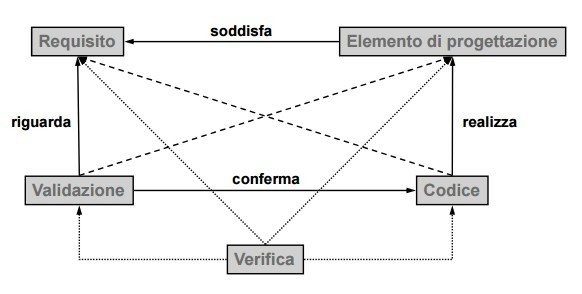
\includegraphics[scale=0.5]{imgs/traceability}
  \caption{Tracciabilità a livello di progetto}
\end{figure}

% TODO  mettere in Progettazione
% \begin{figure}[h!]
%  \centering
%  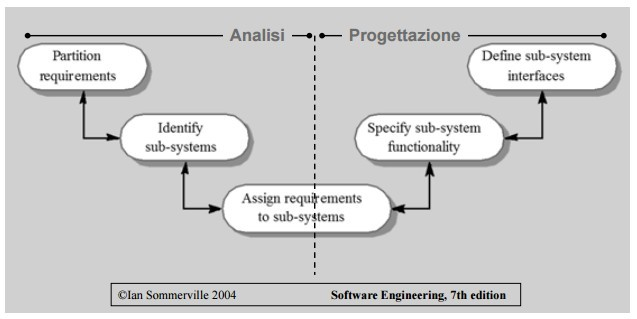
\includegraphics[scale=0.5]{imgs/analysis_vs_design}
%  \caption{Analisi vs progettazione}
%\end{figure}

\subsection{Stato di progresso per SEMAT}
\label{sub:stato_di_progresso_per_semat}

\begin{itemize}
  \item \strong{Conceived}: il commettente è identificato e gli
    stakeholder vedono sufficiente opportunità per il progetto;
  \item \strong{Bounded}: i bisogni sono chiari, i meccanismi di
    gestione dei requisiti (configurazione e cambiamento) sono
    fissati;
  \item \strong{Coherent}: i requisiti sono classificati e quelli
    essenziali (obbligatori) sono chiati e ben definiti;
  \item \strong{Acceptable}: i requisiti fissati definiscono un
    sistema soddisfacente per gli stakeholder;
  \item \strong{Addressed}: il prodotto soddisfa i principali
    requisiti al punto da poter meritare rilascio e uso;
  \item \strong{Fulfilled}: il prodotto soddisfa abbastanza requisiti
    da meritare la piena approvazione degli stakeholder.
\end{itemize}
